\documentclass{article}
\usepackage{iclr2026_conference,times}
\input{math_commands.tex}

\usepackage[T1]{fontenc}
\usepackage{amsmath}
\usepackage{amssymb}
\usepackage{amsthm}
\usepackage{booktabs}
\usepackage{graphicx}
\usepackage{hyperref}
\usepackage{url}

\title{When World Tokens Lie:\\Best-of-$N$ Inference Laws for Tokenized World Models}

% Leave \iclrfinalcopy commented for anonymous review submissions.
\author{Anonymous Authors\\Paper under double-blind review}

\newcommand{\bon}{Best-of-$N$}
\newcommand{\twma}{token-likelihood physical aliasing}
\newcommand{\real}{\mathrm{real}}
\newcommand{\tok}{\mathrm{tok}}

\newtheorem{theorem}{Theorem}

\begin{document}
\maketitle

\begin{abstract}
Tokenized world models compress continuous observations or states into discrete codebook tokens and predict future token sequences. This paper studies a test-time selection question: what happens when a planner samples $N$ token futures and executes the one with the highest internal token score? We show, in controlled tokenized/VQ settings, that larger $N$ can improve selected token likelihood while worsening real decoded utility when the codebook aliases physically distinct futures. We call this \twma{}. We give an exact finite, tie-aware \bon{} law for the selected real-utility curve and validate it by Monte Carlo with mean absolute error $0.00276$. In the main controlled run, raw selection at $N=64$ raises selected token likelihood to $1.386$ while real utility falls to $0.0556$ and alias/physical-violation rates reach $1.0$. A combined token-specific repair raises real utility to $0.629$ and drops both rates to $0.0$, while an oracle reaches $0.957$, leaving a clear gap. The results are diagnostic rather than universal: they do not establish external benchmark performance, hardware deployment evidence, or a general indictment of tokenized world models.
\end{abstract}

\section{Introduction}

Discrete world tokens are appealing because they turn continuous, high-dimensional prediction into a compact symbolic or codebook-indexed sequence problem. A tokenizer can absorb visual detail, a learned transition model can predict future token sequences, and a planner can search over token futures rather than raw states. This pattern appears in VQ-style representation learning, latent world models, and model-based planning systems that separate a compact predictive state from downstream selection.

The same bottleneck creates a planning-specific risk. A token future can be likely under the token model while representing several physically different decoded futures. If the internal score sees only the token sequence, decoded reward, or a token critic, it can assign high score to a future whose real execution is low value because hidden modes, physical validity, or decoder consistency were collapsed by the codebook. We study this as \emph{\twma{}}.

\bon{} selection stresses the issue. A planner samples $N$ candidate futures and selects the highest-scoring one. Increasing $N$ concentrates selection on the upper tail of the score distribution. When the score tail is aligned with real utility, this is useful. When the score tail is physically aliased, larger $N$ can select invalid decoded futures more reliably. The failure is therefore not ``more samples are bad''; it is ``more samples search harder through whatever score tail the token model exposes.''

This paper is a diagnosis-and-repair package for that mechanism. The contribution is deliberately scoped:

\begin{enumerate}
\item We formalize finite token-future selection and give an exact tie-aware \bon{} law for the expected selected real utility of any fixed empirical candidate pool.
\item We identify \twma{} as a concrete failure mode in which token likelihood rises while decoded/executed utility falls.
\item We provide controlled VQ/tokenized evidence, including learned codebook artifacts, codebook-size sweeps, decode-validity diagnostics, and exact-law validation.
\item We test token-specific repairs: codebook uncertainty, alias detection, decode-consistency penalties, physical-validity filtering, rare-mode reweighting, and a small token-to-real pilot calibrator.
\item We package the evidence with an audit discipline that limits claims to controlled settings where aliasing is measurable or pilot labels are collected.
\end{enumerate}

Our claim is not that tokenized world models are broadly flawed, nor that \bon{} is broadly unsafe. The claim is narrower and testable: if the selected score aliases physical utility, high-$N$ selection can amplify the aliasing tail; token-specific diagnostics and pilot calibration can repair this in controlled detectable cases.

\section{Setup}
\label{sec:setup}

Let $x_{0:H}$ denote a physical future and $z_{0:H}=q_\phi(x_{0:H})$ its tokenized representation under a learned codebook. A tokenized world model samples future token sequences from a generator $p_\theta(z_{1:H}\mid z_0,a_{0:H})$ or from an induced candidate pool. A decoder or downstream evaluator maps tokens back to predicted observations, rewards, or constraints.

For each candidate future $c_i$, we distinguish three quantities:
\begin{itemize}
\item a token score $S_i$, such as token likelihood, decoded reward, or a learned token critic;
\item a real utility $R_i$, measured after decoding or executing the corresponding physical future with hidden-mode and validity penalties;
\item diagnostics $D_i$, including alias probability, quantization error, decode-consistency error, physical-violation indicators, and rare-token statistics.
\end{itemize}

The separation between $S_i$ and $R_i$ is essential. In the controlled environment used here, the tokenizer is trained on observable coordinates while a hidden physical mode influences real utility. This makes it possible for multiple physical futures to share token cells or near-identical token scores while differing in validity and utility. We call a candidate \emph{aliased} when its token representation hides a physically important distinction that affects $R_i$ but is weakly represented in $S_i$.

\bon{} selection draws $N$ candidates independently from a finite empirical pool and returns an index with maximal score, breaking score ties uniformly. The selected real utility is $R^{\mathrm{sel}}_N$. We study the curve
\[
N \mapsto \mathbb{E}[R^{\mathrm{sel}}_N],
\]
and compare it for raw token scores, repaired scores, and an oracle real-utility score.

\section{Exact Finite Law}
\label{sec:law}

The central law is finite-population, tie-aware, and score-agnostic. It applies to token likelihood, a repaired diagnostic score, an oracle score, or any other scalar selector.

\begin{theorem}[Tie-aware finite \bon{} law]
Consider a finite candidate pool $\{(S_i,R_i)\}_{i=1}^m$. Partition the candidates into score-tie groups $g$ sorted by increasing score. Let $L_g$ be the number of candidates with score strictly lower than group $g$, let $U_g$ be the number of candidates with score no higher than group $g$, and let $\bar R_g$ be the mean real utility within group $g$. If $N$ candidates are sampled iid uniformly from the pool and the highest-score tie group is broken uniformly, then
\begin{equation}
\mathbb{E}[R^{\mathrm{sel}}_N]
= \sum_g \bar R_g
\left[
\left(\frac{U_g}{m}\right)^N
- \left(\frac{L_g}{m}\right)^N
\right].
\label{eq:finite-law}
\end{equation}
\end{theorem}

The proof is a one-line decomposition over the event that the maximum sampled score falls in group $g$; Appendix~\ref{app:proof} gives the details. Equation~\ref{eq:finite-law} immediately explains both success and failure. The expected selected score is nondecreasing in $N$ because the sample maximum is nondecreasing. The expected selected real utility has no such monotonicity unless high-score groups also have high real utility. A low-utility top score group becomes more likely as $N$ grows.

The law is not asymptotic and does not assume continuous scores. This matters for tokenized world models because ties and near-ties are common: codebook cells merge many continuous states, token likelihoods can be quantized or smoothed, and decoded reward can saturate.

\section{Token-Specific Diagnostics and Repairs}
\label{sec:method}

The repair methods target the token bottleneck rather than generic score smoothing. Each candidate receives the raw token score
\[
S_i^{\mathrm{raw}} = 0.70 \cdot \ell_i^{\tok}
 + 0.35 \cdot \hat r_i^{\tok}
 - 0.04 \cdot e_i^{\mathrm{q}}
 + \epsilon_i,
\]
where $\ell_i^{\tok}$ is token likelihood, $\hat r_i^{\tok}$ is decoded reward, $e_i^{\mathrm{q}}$ is quantization error, and $\epsilon_i$ is small score noise in the controlled generator. Real utility is evaluated separately and penalizes hidden-mode mismatch and physical invalidity.

We evaluate six repair families.

\paragraph{Codebook uncertainty.}
This score penalizes token-level alias probability and normalized quantization error. It asks whether the selected candidate lies in a codebook cell known to merge hidden modes or reconstruct poorly.

\paragraph{Decode consistency.}
This score penalizes disagreement between token-implied futures and decoded physical futures, together with physical-violation scores. It is designed for cases where the token model predicts a plausible code sequence that decodes into an impossible trajectory.

\paragraph{Physical filter.}
This score applies a hard penalty when a candidate crosses a physical-violation threshold, then applies a lighter alias penalty to the remaining candidates. In this paper the filter uses generated diagnostics; in a deployment it would require task-specific validity checks.

\paragraph{Rare-mode reweighting.}
This score rewards rare tokens while penalizing alias and violation diagnostics. It tests whether the raw score is discarding rare but valid high-utility futures.

\paragraph{Token-to-real pilot calibration.}
A small ridge calibrator maps token diagnostics to real utility using a pilot fraction of labeled candidates. This is the only repair that uses real-utility labels. It is therefore powerful but not free.

\paragraph{Combined repair and gate.}
The combined score averages codebook uncertainty, decode consistency, physical filtering, and pilot calibration with fixed weights. A deployment gate inspects high-$N$ alias rate, physical-violation rate, raw utility drop, repair gain, and exact-law error. In the main run the gate returns \texttt{collect\_pilot\_labels}, because pilot calibration repairs a harmful high-$N$ tail but the raw selector is unsafe.

\section{Experiments}
\label{sec:experiments}

All experiments are CPU-local controlled experiments. The goal is to isolate the token-tail mechanism, not to claim external benchmark or hardware performance. The repository includes every primary artifact under \path{results/} and \path{figures/}.

\paragraph{World-token construction.}
We generate synthetic physical observations with an omitted hidden mode, train a small VQ tokenizer, and estimate token frequency, transition statistics, quantization error, and alias probability. The main learned artifact uses codebook size $8$, collision rate $0.232$, mean quantization error $0.120$, token entropy $2.946$, and transition self-probability $0.137$.

\paragraph{Candidate pools.}
For each of $150$ pools with $64$ candidates, the generator emits a mixture of valid candidates, aliased candidates, rare-good candidates, and low-quality candidates. The raw score favors high token likelihood and decoded reward. Real utility is clipped to $[-0.05,1.0]$ after hidden-mode and physical-validity penalties. We evaluate $N\in\{1,2,4,8,16,32,64\}$.

\paragraph{Artifacts.}
The main metrics are in \path{results/metrics_main.csv}; tail autopsy rows are in \path{results/tail_autopsy.csv}; exact-law validation is in \path{results/exact_law_validation.json}; and claim status is in \path{results/claims_status.json}. Figure~\ref{fig:failure} shows the raw failure curve.

\begin{figure}[t]
\centering
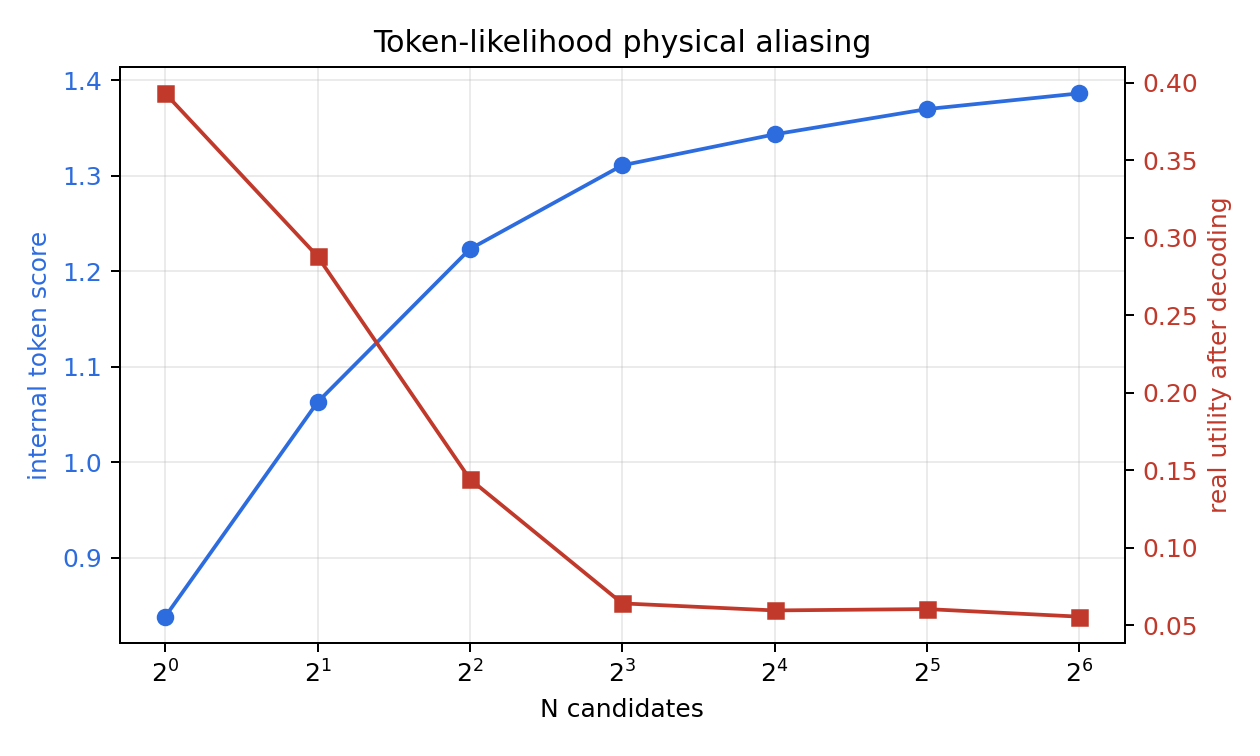
\includegraphics[width=0.82\linewidth]{figures/figure1_token_likelihood_physical_aliasing.png}
\caption{Raw \bon{} selection amplifies token-likelihood physical aliasing. As $N$ grows, selected token likelihood rises, but selected real utility falls because the high-score tail is dominated by aliased and physically invalid decoded futures.}
\label{fig:failure}
\end{figure}

\subsection[Raw High-N Selection Selects the Wrong Tail]{Raw High-$N$ Selection Selects the Wrong Tail}
\label{sec:raw-results}

Raw token selection looks better if one watches only token likelihood. At $N=1$, selected token likelihood is $0.838$ and selected real utility is $0.393$. At $N=64$, selected token likelihood rises to $1.386$, but real utility falls to $0.0556$. Alias rate and physical-violation rate both reach $1.0$, and decode-consistency error reaches $0.613$.

This is exactly the tail effect predicted by Equation~\ref{eq:finite-law}. The selected score improves because the maximum score improves. The selected real utility falls because the upper score group is dominated by aliased candidates.

\begin{table}[t]
\caption{Main selected-tail statistics. Raw high-$N$ selection improves token likelihood while collapsing real utility. Repairs reduce detected aliasing and physical invalidity, but oracle selection remains substantially better.}
\label{tab:main}
\centering
\small
\begin{tabular}{@{}llrrrrr@{}}
\toprule
Selector & $N$ & Token likelihood & Real utility & Alias rate & Violation rate & Decode error \\
\midrule
Raw token score & 1 & 0.838 & 0.393 & 0.387 & 0.467 & 0.450 \\
Raw token score & 64 & 1.386 & 0.0556 & 1.000 & 1.000 & 0.613 \\
Combined repair & 64 & 0.755 & 0.629 & 0.000 & 0.000 & 0.274 \\
Pilot calibrator & 64 & 0.463 & 0.819 & 0.000 & 0.000 & 0.299 \\
Oracle real utility & 64 & 0.488 & 0.957 & 0.000 & 0.000 & 0.317 \\
\bottomrule
\end{tabular}
\end{table}

\subsection{Repair Helps, But Does Not Close the Oracle Gap}
\label{sec:repair-results}

Figure~\ref{fig:repair} compares raw selection, individual repairs, combined repair, the pilot calibrator, and oracle selection. The combined repair raises real utility at $N=64$ from $0.0556$ to $0.629$ and drops both alias and violation rates from $1.0$ to $0.0$. The standalone pilot calibrator reaches $0.819$, showing the value of small real-utility labels in this controlled setting. Oracle real-utility selection reaches $0.957$.

The gap is important. The combined repair leaves an oracle gap of $0.327$ at $N=64$, and even the pilot calibrator leaves a gap of $0.138$. We therefore treat repair as conditional evidence for detectable aliasing, not as a universal fix.

\begin{figure}[t]
\centering
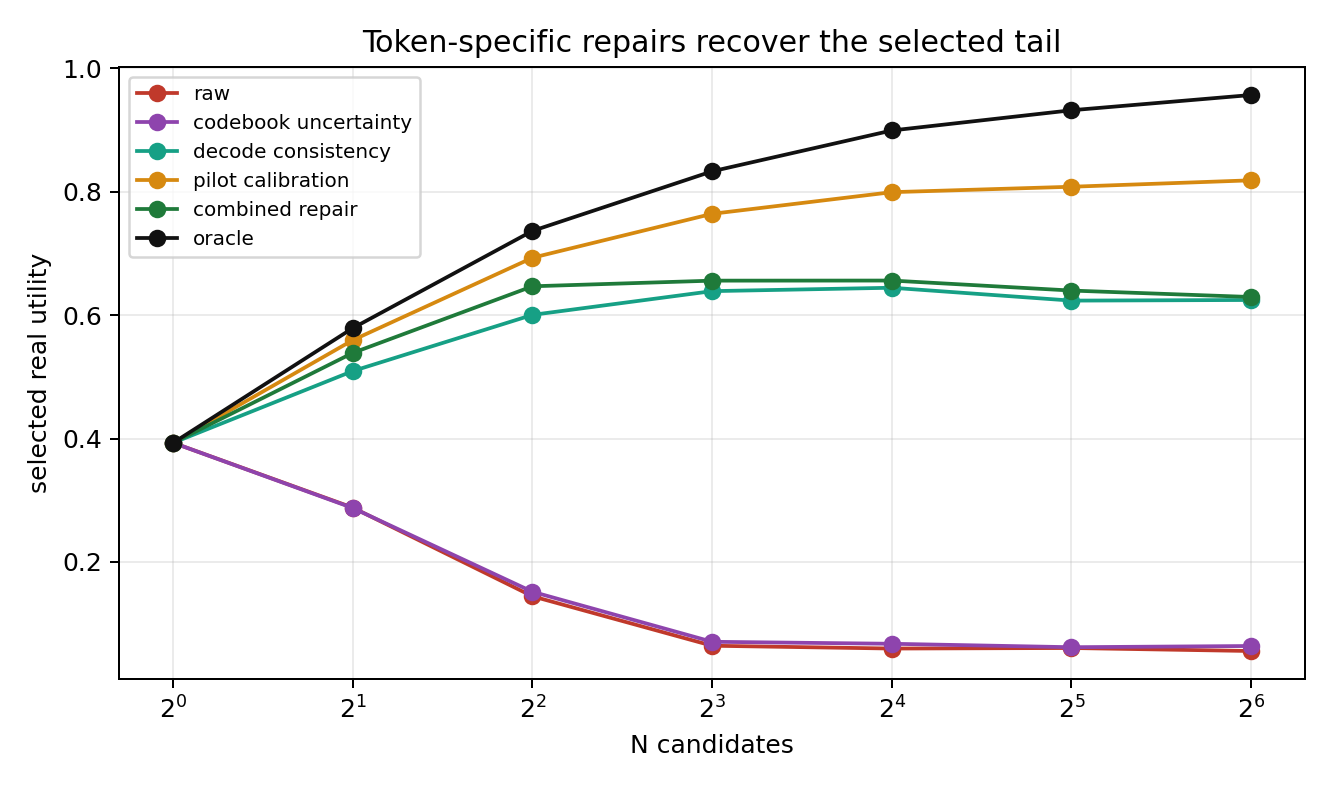
\includegraphics[width=0.86\linewidth]{figures/figure2_repair_comparison.png}
\caption{Token-specific repairs can redirect high-$N$ selection away from aliased futures. The strongest label-based pilot calibrator is intentionally separated from hand-coded diagnostics because it spends real-utility labels.}
\label{fig:repair}
\end{figure}

\subsection{Codebook Bottlenecks and Decode Diagnostics}
\label{sec:diagnostics-results}

The codebook-size sweep tests whether the failure is merely a small-codebook artifact. As codebook size increases from $4$ to $24$, mean quantization error decreases from $0.159$ to $0.070$, but collision rates remain near $0.24$--$0.27$ because the hidden physical mode remains omitted. Raw $N=64$ real utility stays low, between $0.038$ and $0.089$, while combined repair gains remain between $0.553$ and $0.622$.

Decode diagnostics localize the selected bad tail. In the tail autopsy, raw $N=64$ selections are aliased candidates with high token likelihood, high physical-violation scores, and low real utility. Combined repair selections are mostly valid candidates with lower violation scores. Figure~\ref{fig:bottleneck-diagnostics} shows both the codebook sweep and the diagnostic distributions.

\begin{figure}[t]
\centering
\begin{minipage}{0.49\linewidth}
\centering
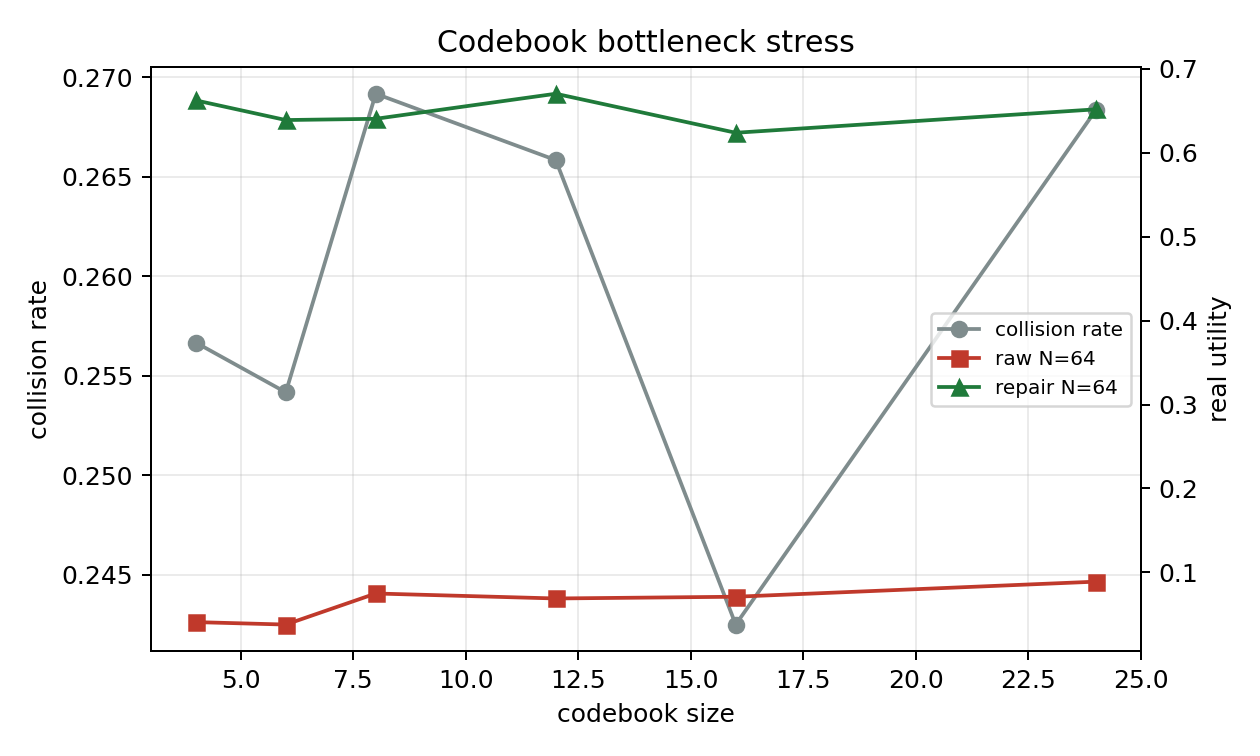
\includegraphics[width=\linewidth]{figures/figure3_codebook_bottleneck_curve.png}
\end{minipage}
\hfill
\begin{minipage}{0.49\linewidth}
\centering
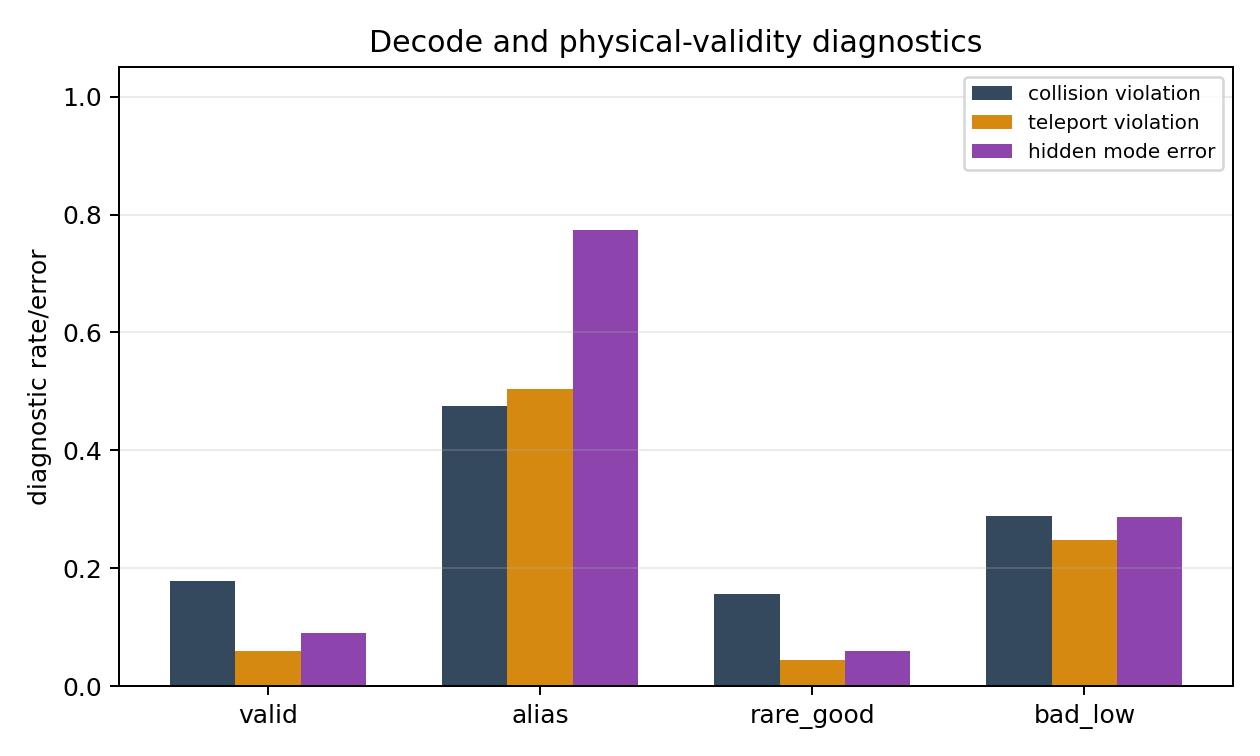
\includegraphics[width=\linewidth]{figures/figure4_decode_validity_diagnostics.png}
\end{minipage}
\caption{Left: increasing codebook size reduces quantization error but does not remove hidden-mode collisions in this controlled setup. Right: token-specific diagnostics separate raw high-score aliased candidates from repaired valid selections.}
\label{fig:bottleneck-diagnostics}
\end{figure}

\subsection{Exact-Law Validation}
\label{sec:law-results}

For fixed empirical pools, Equation~\ref{eq:finite-law} gives the expected selected real utility exactly. We validate the implementation against Monte Carlo draws over $N\in\{1,2,4,8,16,32,64\}$. Mean absolute error is $0.00276$ and maximum error is $0.00779$, consistent with simulation noise. Figure~\ref{fig:law} plots exact and Monte Carlo curves.

\begin{figure}[t]
\centering
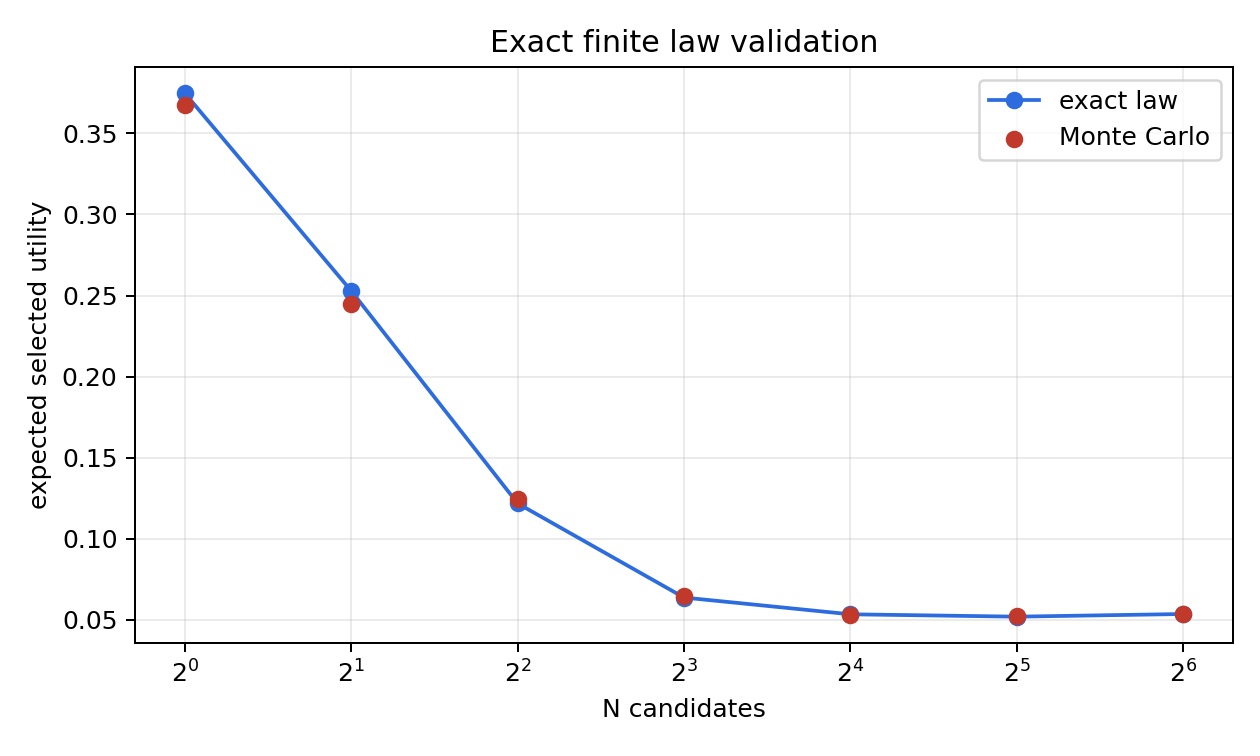
\includegraphics[width=0.78\linewidth]{figures/figure5_exact_law_validation.png}
\caption{The finite tie-aware law predicts the selected real-utility curve for the fixed empirical token-future pool. The residual is Monte Carlo estimation error, not an asymptotic approximation gap.}
\label{fig:law}
\end{figure}

\section{Related Work}
\label{sec:related}

\paragraph{Discrete and tokenized representations.}
Vector-quantized autoencoders introduced learned discrete latent codebooks for neural representation learning \citep{oord2017neural}. Later work used discrete latents for high-fidelity image and video generation \citep{razavi2019generating,esser2021taming}. Our focus is not generation quality; it is the planning consequence of selecting from token-future score tails when a codebook cell hides physically relevant distinctions.

\paragraph{World models and model-based planning.}
World models learn predictive latent dynamics for decision making \citep{ha2018world,hafner2019learning,hafner2020dream}. Model-based RL and MPC systems use learned dynamics to plan by sampling or optimizing candidate futures \citep{chua2018deep,nagabandi2018neural,williams2017information}. We study a narrow inference-time selection law inside such systems: the generator can be held fixed while the selected score tail changes with $N$.

\paragraph{Reranking, verifiers, and \bon{} selection.}
Sampling many candidates and selecting with a verifier, reward model, or critic is common in sequence generation and decision systems \citep{cobbe2021training,nakano2021webgpt,stiennon2020learning}. The same pattern appears in planning as trajectory sampling plus scoring. Our contribution is to make the selected real-utility curve finite and auditable for tokenized world futures, especially under score-utility aliasing.

\paragraph{Calibration and safety filtering.}
Calibration methods relate model scores to empirical outcomes \citep{zadrozny2002transforming,guo2017calibration}. Selective prediction and safety filters abstain or constrain decisions when confidence or validity checks fail \citep{geifman2017selective,wabersich2021predictive}. Our deployment gate is in this spirit, but specialized to token-future diagnostics: alias rate, decode consistency, physical validity, repair gain, and pilot token-to-real labels.

\section{Limitations and Claim Discipline}
\label{sec:limits}

The experiments are synthetic and controlled. The tokenizer, hidden mode, candidate generator, and validity penalties are designed to expose the mechanism. This is useful for diagnosis, but it is not an external benchmark result and not hardware deployment evidence. The learned VQ artifact is small, and the candidate pools are generated from a controlled mixture rather than a large-scale embodied world model.

The repairs are conditional. Codebook uncertainty helps only when aliasing is reflected in codebook statistics. Decode consistency helps only when invalid decoded futures are detectable. Physical filtering requires a meaningful validity check. Pilot calibration requires representative real-utility labels and can drift if the deployment distribution changes. The deployment gate therefore returns \texttt{collect\_pilot\_labels} in the main run rather than declaring raw high-$N$ selection safe.

The finite law is exact for a fixed empirical pool and iid sampling with uniform tie breaking. It does not by itself solve distribution shift, adaptive candidate generation, correlated rollouts, or misspecified real utility. Those cases require fresh audited pools or stronger assumptions.

\section{Conclusion}

\bon{} planning over world tokens is a tail-selection problem. Increasing $N$ reliably searches the upper tail of the token score, but whether that improves real utility depends on whether the score tail is physically meaningful. In our controlled tokenized/VQ setting, raw high-$N$ selection amplifies \twma{}: token likelihood rises, real utility falls, and selected futures become aliased and physically invalid. The exact finite law predicts this curve, and token-specific diagnostics plus pilot calibration repair the detectable case while leaving an honest oracle gap. The practical message is simple: before increasing $N$ for tokenized world-model planning, audit the token-score tail against real utility or use a gate that asks for pilot labels, repair, or abstention.

\section*{Reproducibility Statement}
The repository includes source code, tests, generated CSV/JSON artifacts, figures, and this LaTeX source. The main reproduction commands are \texttt{bash scripts/run\_all.sh}, \texttt{bash scripts/run\_claim\_audit.sh}, \texttt{pytest}, and \texttt{powershell -ExecutionPolicy Bypass -File paper/iclr/build.ps1}. Appendix~\ref{app:commands} maps the paper build and audit commands.

\section*{Ethics and Impact Statement}
This work uses synthetic CPU-local experiments and does not use human subjects, private data, deployed robots, or safety-critical hardware trials. The main risk is over-interpreting controlled diagnostic evidence as deployment certification. The paper explicitly limits the claim and recommends task-specific audits before using high-$N$ selection in new systems.

\section*{LLM Usage Statement}
Large language models were used for drafting and packaging assistance. The authors are responsible for the claims, code, citations, and final text. Numerical claims are taken from tracked repository artifacts.

\phantomsection\label{maintextend}
\bibliography{references}
\bibliographystyle{iclr2026_conference}

\appendix
\section{Proof of the Finite Law}
\label{app:proof}

Let the finite pool contain $m$ candidates and let group $g$ contain all candidates with one tied score value. The event that the selected maximum score lies in group $g$ is the event that all $N$ iid draws have score no higher than group $g$ and not all draws have score strictly lower than group $g$. Since $U_g$ candidates have score no higher than the group and $L_g$ candidates have score strictly lower, the probability of this event is
\[
\left(\frac{U_g}{m}\right)^N -
\left(\frac{L_g}{m}\right)^N.
\]
Conditional on this event, uniform tie breaking within the selected score group gives expected utility $\bar R_g$. Summing these disjoint events over score groups proves Equation~\ref{eq:finite-law}. Replacing $\bar R_g$ with the group mean score yields the expected selected-score curve.

The law also clarifies why selected real utility can decrease with $N$. If the top score group has lower $\bar R_g$ than lower score groups, then the probability mass on that low-utility group increases with $N$. No smoothness, calibration, or continuous-score assumption is required. This is useful for tokenized world models because codebook scores can be tied, saturated, or quantized.

\section{Controlled Generator Details}
\label{app:details}

The controlled generator is implemented in \path{src/token_alias_tail_audit/simulation.py}. It first builds synthetic observations with an omitted hidden physical mode, fits a small VQ codebook, and estimates per-token frequency, alias probability, quantization error, and transition statistics. Candidate pools are then sampled from four candidate kinds:
\begin{itemize}
\item \texttt{alias}: high token likelihood and decoded reward, high physical violation, hidden-mode error, and low real utility;
\item \texttt{rare\_good}: lower token likelihood, low physical violation, and high real utility;
\item \texttt{bad\_low}: low score and low utility;
\item \texttt{valid}: moderate score, low violation, and moderate utility.
\end{itemize}

The main run uses \VThreePools{} pools, pool size \VThreePoolSize{}, and $N\in\{1,2,4,8,16,32,64\}$. All selectors are evaluated on the same generated candidates. The exact law is validated against Monte Carlo draws from the raw-score empirical pool.

\begin{table}[h]
\caption{Semi-learned VQ artifact used in the main run.}
\label{tab:vq-artifact}
\centering
\small
\begin{tabular}{@{}lr@{}}
\toprule
Quantity & Value \\
\midrule
Codebook size & \VThreeVQCodebookSize{} \\
Collision rate & \VThreeVQCollision{} \\
Mean quantization error & \VThreeVQQuantError{} \\
Token entropy & \VThreeVQEntropy{} \\
Mean transition self-probability & \VThreeVQTransitionSelf{} \\
\bottomrule
\end{tabular}
\end{table}

\section{Repair Score Definitions}
\label{app:repair}

Let $S^{\mathrm{raw}}$, $a$, $q$, $d$, $v$, and $b$ denote raw score, alias probability, quantization error, decode-consistency error, physical violation, and rare-token bonus. The implemented diagnostic scores are
\[
S^{\mathrm{codebook}} = S^{\mathrm{raw}} - 0.85a - 0.25q,
\]
\[
S^{\mathrm{decode}} = S^{\mathrm{raw}} - 0.95d - 0.75v,
\]
\[
S^{\mathrm{filter}} =
\begin{cases}
S^{\mathrm{raw}} - 2.0, & v > 0.45,\\
S^{\mathrm{raw}} - 0.35a, & v \leq 0.45,
\end{cases}
\]
\[
S^{\mathrm{rare}} = S^{\mathrm{raw}} - 0.75a + 0.35b - 0.55v.
\]
The pilot calibrator is a ridge regressor from token diagnostics to real utility, trained on a pilot fraction of generated candidates with a minimum pilot-label floor. The combined repair is
\[
S^{\mathrm{combined}} =
0.15S^{\mathrm{codebook}}
+0.15S^{\mathrm{decode}}
+0.25S^{\mathrm{filter}}
+0.45S^{\mathrm{calibrated}}.
\]
These weights are fixed in the repository implementation and are not tuned per figure.

\section{Additional Diagnostic Figures}
\label{app:figures}

The following figures are included to make the token-specific mechanism visible. They are not external benchmark results; each figure is generated from the controlled local artifacts.

\begin{figure}[H]
\centering
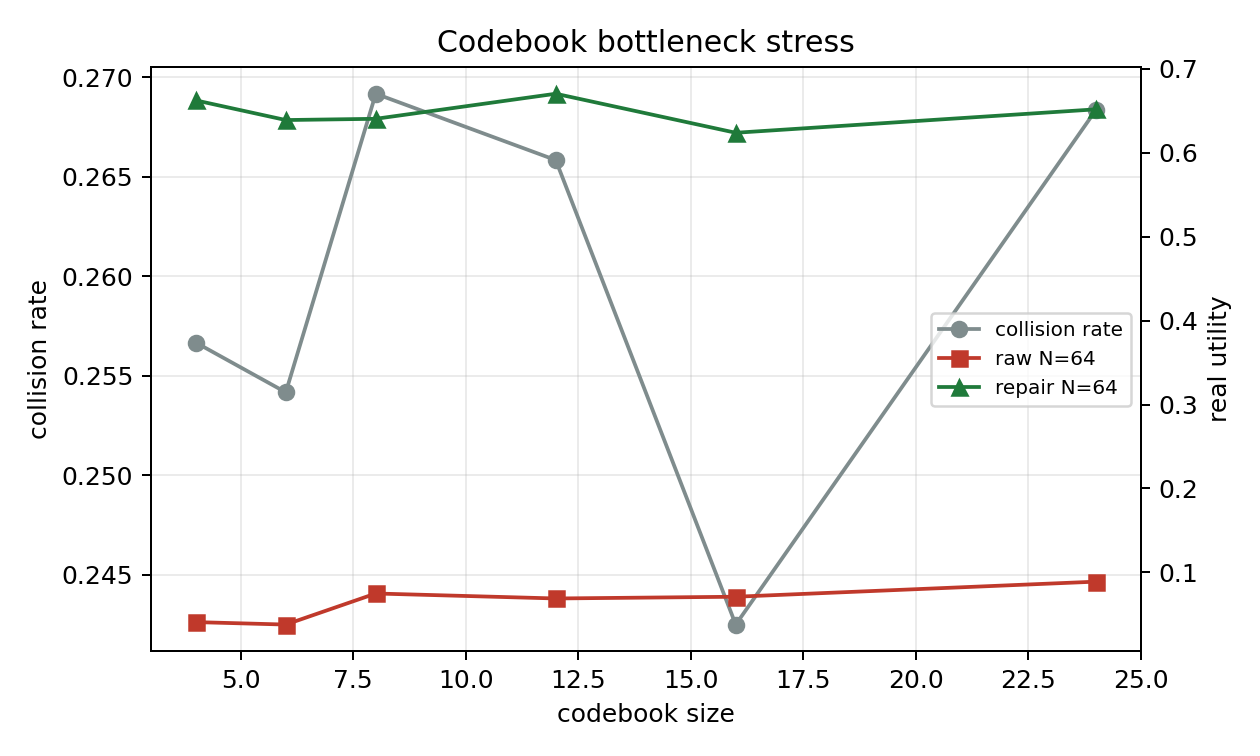
\includegraphics[width=0.86\linewidth]{figures/figure3_codebook_bottleneck_curve.png}
\caption{Codebook bottleneck curve from the original full artifact.}
\label{fig:appendix-codebook}
\end{figure}

\begin{figure}[H]
\centering
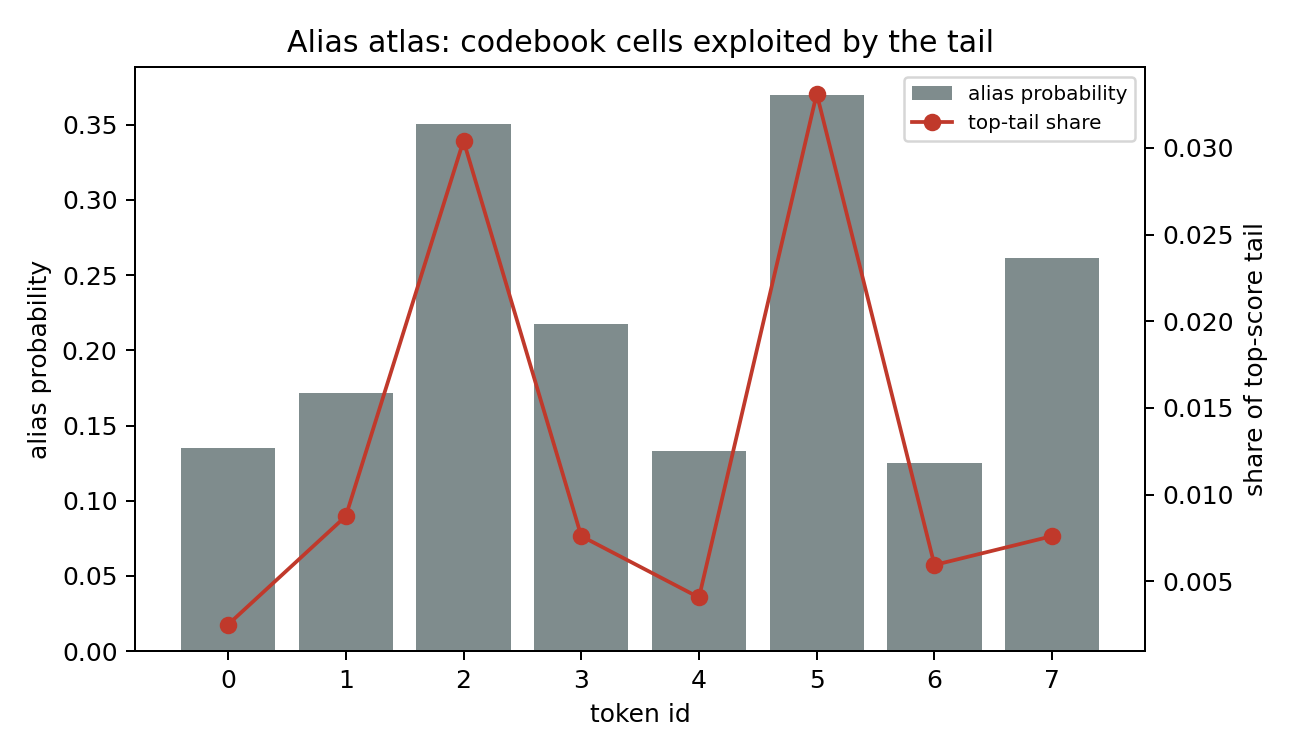
\includegraphics[width=0.86\linewidth]{figures/figure6_alias_atlas.png}
\caption{Alias atlas for the controlled tokenized world model. Raw high-score selection concentrates in token regions where hidden-mode aliasing and decoded physical invalidity are high.}
\label{fig:alias-atlas}
\end{figure}

\begin{figure}[H]
\centering
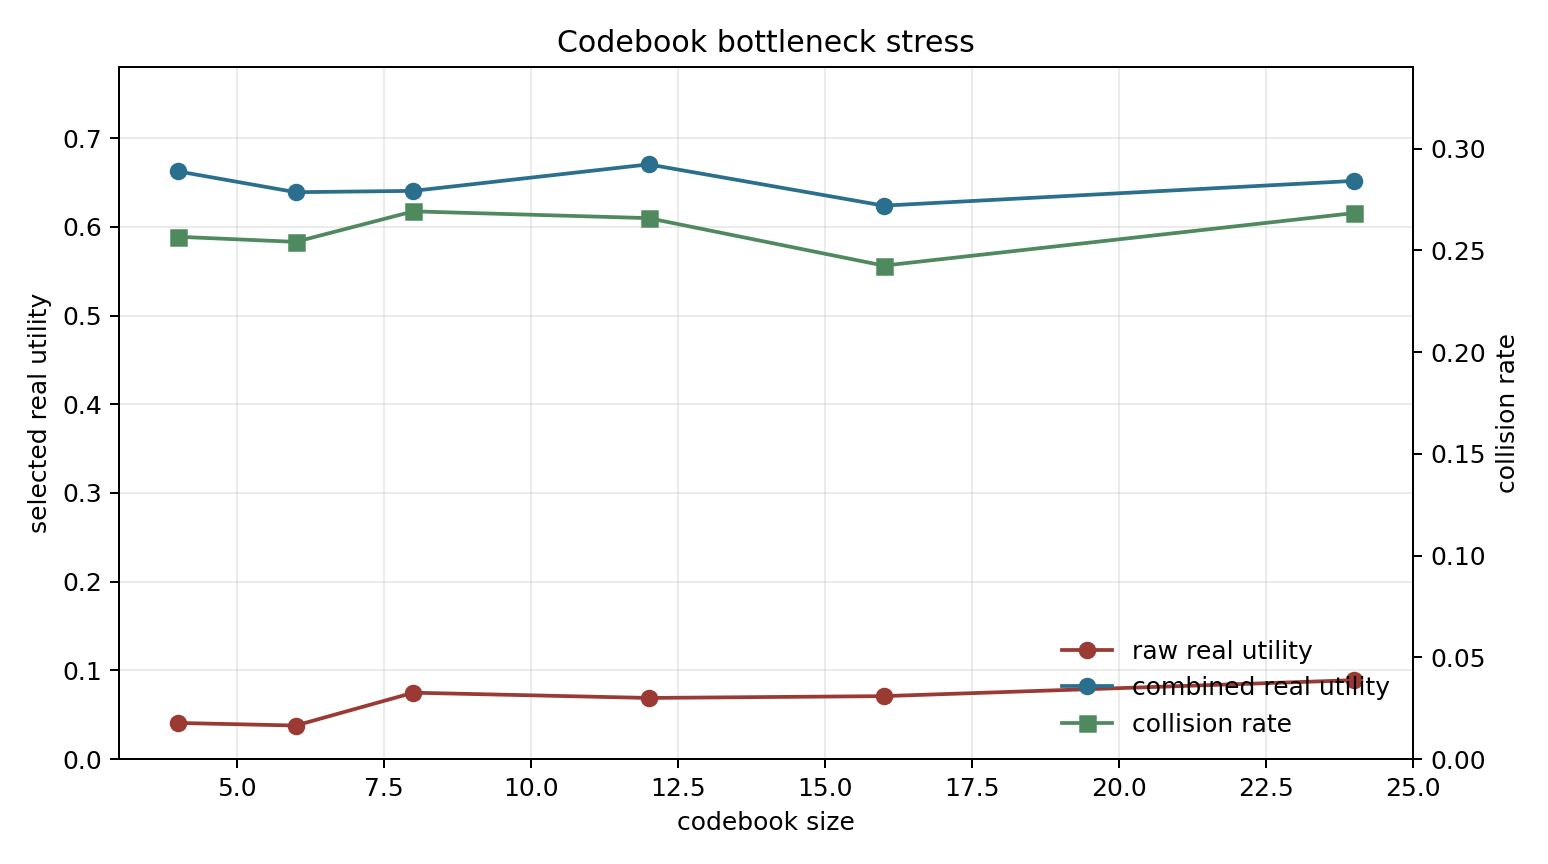
\includegraphics[width=0.86\linewidth]{figures/figure9_v3_codebook_stress.png}
\caption{V3 codebook stress synthesis. Raw high-budget utility remains low across the codebook-size sweep even as quantization error changes.}
\label{fig:appendix-v3-codebook}
\end{figure}

\begin{figure}[H]
\centering
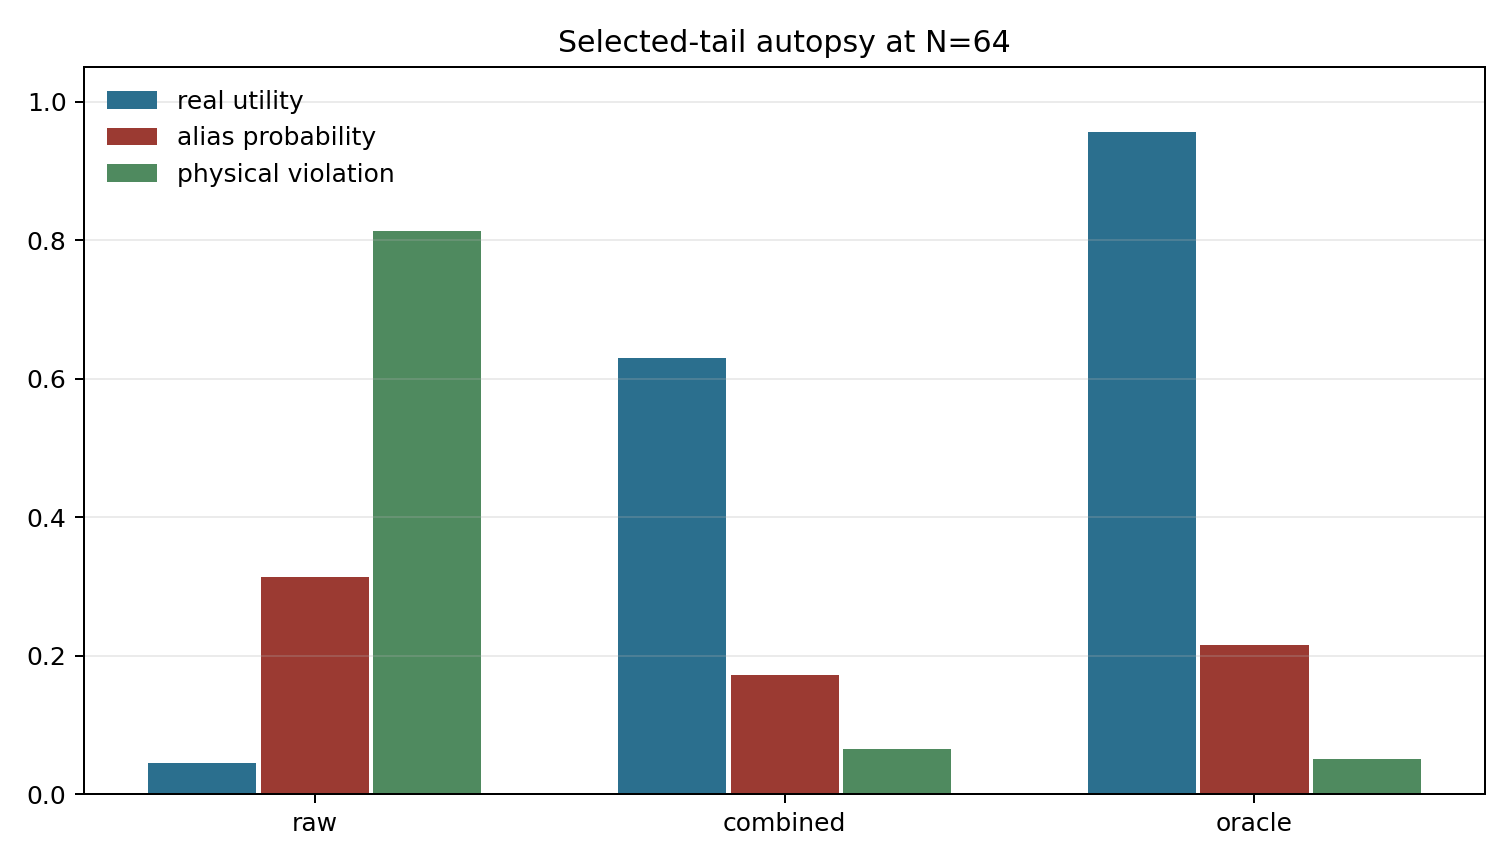
\includegraphics[width=0.86\linewidth]{figures/figure10_v3_tail_autopsy.png}
\caption{V3 tail autopsy. Raw high-budget selection chooses alias-heavy candidates; combined repair shifts the selected tail toward valid futures; oracle selects the highest real utility.}
\label{fig:appendix-v3-tail}
\end{figure}

\begin{figure}[H]
\centering
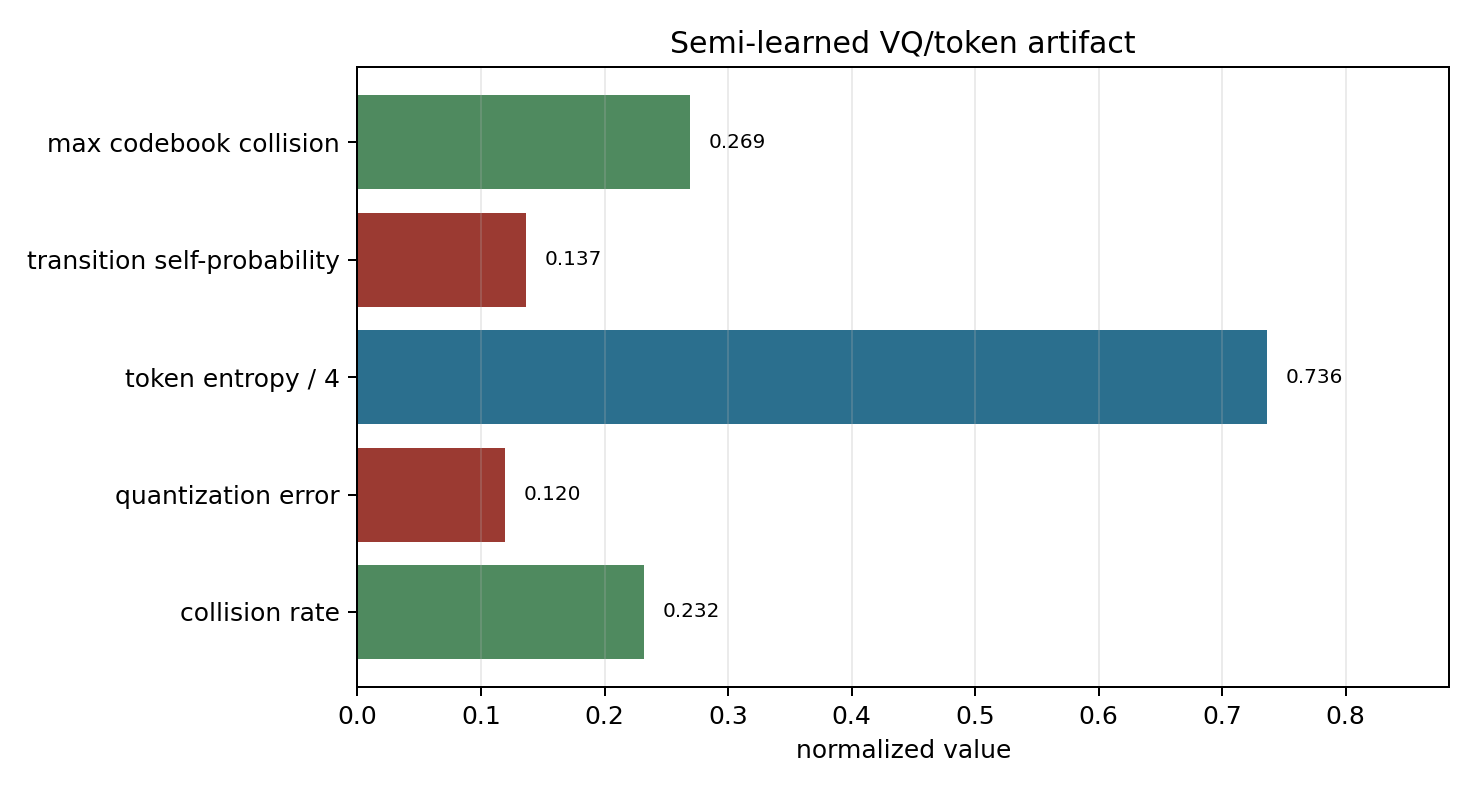
\includegraphics[width=0.86\linewidth]{figures/figure11_v3_vq_artifact.png}
\caption{V3 semi-learned VQ artifact summary.}
\label{fig:appendix-v3-vq}
\end{figure}

\section{Selector Table}
\label{app:selectors}

\begin{table}[H]
\caption{High-budget selector interpretation. The paper separates label-spending calibration from no-label diagnostics and oracle upper bounds.}
\label{tab:selectors}
\centering
\small
\begin{tabular}{@{}p{0.23\linewidth}p{0.24\linewidth}p{0.20\linewidth}p{0.23\linewidth}@{}}
\toprule
Selector & Uses & Strength & Limitation \\
\midrule
Raw token score & token likelihood, decoded reward & tests failure & unsafe when high-score tail aliases utility \\
Codebook uncertainty & alias probability, quantization error & token-specific diagnostic & weak if alias cells still dominate likelihood \\
Decode consistency & decoded physical agreement & strong controlled repair & requires meaningful decode diagnostics \\
Physical filter & physical-violation threshold & strong controlled repair & needs task-specific validity checks \\
Rare-mode reweighting & rare-token bonus plus penalties & tests rare valid modes & rare tokens can be mixed quality \\
Pilot calibrator & token diagnostics plus labels & strongest repair here & spends real-utility labels and can drift \\
Combined repair & fixed blend of diagnostics and calibration & controlled repair stack & still below oracle \\
Oracle & real utility & upper bound & not deployable evidence \\
\bottomrule
\end{tabular}
\end{table}

\section{Full Cached Evidence Tables}
\label{app:full-evidence}

This appendix section exposes the complete cached evidence behind the compact main-text scorecard. The intent is to make the paper harder to attack on cherry-picking grounds: every selector, every budget, the codebook sweep, and the selected high-budget tails are listed directly from the repository artifacts.

Table~\ref{tab:v3-full-curves} is the full selected-tail curve for all selectors and all candidate budgets. It shows the central non-monotonicity in its most direct form: raw token-score selection raises selected token likelihood as the budget grows, while selected real utility collapses and the selected tail becomes entirely aliasing and physically invalid. The same table also separates the repairs by evidence cost. Decode consistency and physical filtering reduce aliasing without real-utility labels; the pilot calibrator spends labels and therefore gives the strongest controlled repair; the oracle is retained only as an unreachable upper bound.

% Auto-generated by scripts/prepare_v3_evidence.py
\begin{table}[H]
\centering
\scriptsize
\setlength{\tabcolsep}{3pt}
\caption{Full selected-tail curves for the controlled tokenized candidate pools, rows 1--14.}\label{tab:v3-full-curves}
\begin{tabular}{@{}lrrrrrr@{}}
\toprule
Selector & $N$ & token likelihood & real utility & alias & violation & oracle gap \\
\midrule
raw & 1 & 0.838 & 0.393 & 0.387 & 0.467 & 0.000 \\
raw & 2 & 1.063 & 0.288 & 0.627 & 0.633 & 0.291 \\
raw & 4 & 1.223 & 0.144 & 0.853 & 0.853 & 0.592 \\
raw & 8 & 1.311 & 0.064 & 0.980 & 0.980 & 0.769 \\
raw & 16 & 1.344 & 0.060 & 1.000 & 1.000 & 0.840 \\
raw & 32 & 1.370 & 0.061 & 1.000 & 1.000 & 0.872 \\
raw & 64 & 1.386 & 0.056 & 1.000 & 1.000 & 0.901 \\
codebook & 1 & 0.838 & 0.393 & 0.387 & 0.467 & 0.000 \\
codebook & 2 & 1.062 & 0.287 & 0.627 & 0.633 & 0.292 \\
codebook & 4 & 1.214 & 0.152 & 0.853 & 0.853 & 0.585 \\
codebook & 8 & 1.299 & 0.071 & 0.980 & 0.980 & 0.763 \\
codebook & 16 & 1.326 & 0.067 & 0.993 & 0.993 & 0.832 \\
codebook & 32 & 1.341 & 0.062 & 1.000 & 1.000 & 0.870 \\
codebook & 64 & 1.358 & 0.064 & 1.000 & 1.000 & 0.893 \\
\bottomrule
\end{tabular}
\end{table}

\begin{table}[H]
\centering
\scriptsize
\setlength{\tabcolsep}{3pt}
\caption{Full selected-tail curves for the controlled tokenized candidate pools, rows 15--28.}
\begin{tabular}{@{}lrrrrrr@{}}
\toprule
Selector & $N$ & token likelihood & real utility & alias & violation & oracle gap \\
\midrule
decode & 1 & 0.838 & 0.393 & 0.387 & 0.467 & 0.000 \\
decode & 2 & 0.820 & 0.509 & 0.260 & 0.260 & 0.070 \\
decode & 4 & 0.758 & 0.601 & 0.113 & 0.113 & 0.136 \\
decode & 8 & 0.726 & 0.639 & 0.020 & 0.020 & 0.194 \\
decode & 16 & 0.753 & 0.644 & 0.007 & 0.007 & 0.255 \\
decode & 32 & 0.781 & 0.624 & 0.000 & 0.000 & 0.309 \\
decode & 64 & 0.803 & 0.625 & 0.000 & 0.000 & 0.332 \\
filter & 1 & 0.838 & 0.393 & 0.387 & 0.467 & 0.000 \\
filter & 2 & 0.765 & 0.536 & 0.187 & 0.187 & 0.043 \\
filter & 4 & 0.716 & 0.626 & 0.040 & 0.040 & 0.111 \\
filter & 8 & 0.730 & 0.628 & 0.000 & 0.000 & 0.206 \\
filter & 16 & 0.776 & 0.620 & 0.000 & 0.000 & 0.279 \\
filter & 32 & 0.810 & 0.620 & 0.000 & 0.000 & 0.312 \\
filter & 64 & 0.836 & 0.617 & 0.000 & 0.000 & 0.340 \\
\bottomrule
\end{tabular}
\end{table}

\begin{table}[H]
\centering
\scriptsize
\setlength{\tabcolsep}{3pt}
\caption{Full selected-tail curves for the controlled tokenized candidate pools, rows 29--42.}
\begin{tabular}{@{}lrrrrrr@{}}
\toprule
Selector & $N$ & token likelihood & real utility & alias & violation & oracle gap \\
\midrule
rare & 1 & 0.838 & 0.393 & 0.387 & 0.467 & 0.000 \\
rare & 2 & 0.938 & 0.407 & 0.440 & 0.447 & 0.172 \\
rare & 4 & 1.002 & 0.361 & 0.500 & 0.500 & 0.376 \\
rare & 8 & 1.032 & 0.332 & 0.533 & 0.533 & 0.501 \\
rare & 16 & 1.053 & 0.328 & 0.533 & 0.533 & 0.571 \\
rare & 32 & 1.090 & 0.322 & 0.560 & 0.560 & 0.610 \\
rare & 64 & 1.141 & 0.281 & 0.620 & 0.620 & 0.675 \\
pilot & 1 & 0.838 & 0.393 & 0.387 & 0.467 & 0.000 \\
pilot & 2 & 0.698 & 0.560 & 0.160 & 0.187 & 0.019 \\
pilot & 4 & 0.609 & 0.693 & 0.040 & 0.040 & 0.044 \\
pilot & 8 & 0.545 & 0.764 & 0.000 & 0.000 & 0.069 \\
pilot & 16 & 0.517 & 0.799 & 0.000 & 0.000 & 0.100 \\
pilot & 32 & 0.488 & 0.808 & 0.000 & 0.000 & 0.124 \\
pilot & 64 & 0.463 & 0.819 & 0.000 & 0.000 & 0.138 \\
\bottomrule
\end{tabular}
\end{table}

\begin{table}[H]
\centering
\scriptsize
\setlength{\tabcolsep}{3pt}
\caption{Full selected-tail curves for the controlled tokenized candidate pools, rows 43--56.}
\begin{tabular}{@{}lrrrrrr@{}}
\toprule
Selector & $N$ & token likelihood & real utility & alias & violation & oracle gap \\
\midrule
combined & 1 & 0.838 & 0.393 & 0.387 & 0.467 & 0.000 \\
combined & 2 & 0.753 & 0.539 & 0.187 & 0.187 & 0.040 \\
combined & 4 & 0.695 & 0.647 & 0.040 & 0.040 & 0.090 \\
combined & 8 & 0.694 & 0.656 & 0.000 & 0.000 & 0.177 \\
combined & 16 & 0.713 & 0.656 & 0.000 & 0.000 & 0.243 \\
combined & 32 & 0.742 & 0.640 & 0.000 & 0.000 & 0.292 \\
combined & 64 & 0.755 & 0.629 & 0.000 & 0.000 & 0.327 \\
oracle & 1 & 0.838 & 0.393 & 0.387 & 0.467 & 0.000 \\
oracle & 2 & 0.711 & 0.579 & 0.167 & 0.200 & 0.000 \\
oracle & 4 & 0.602 & 0.737 & 0.040 & 0.047 & 0.000 \\
oracle & 8 & 0.541 & 0.833 & 0.000 & 0.007 & 0.000 \\
oracle & 16 & 0.513 & 0.899 & 0.000 & 0.000 & 0.000 \\
oracle & 32 & 0.502 & 0.932 & 0.000 & 0.000 & 0.000 \\
oracle & 64 & 0.488 & 0.957 & 0.000 & 0.000 & 0.000 \\
\bottomrule
\end{tabular}
\end{table}


Table~\ref{tab:v3-codebook-sweep} reports the cached codebook-size stress test. This is not used to claim that codebook size is irrelevant. It is used to show that, in this generator, merely changing the bottleneck size does not remove the selected-tail pathology: raw high-budget utility remains low across the sweep, and a token-aware repair keeps a large gain in every tested setting.

% Auto-generated by scripts/prepare_v3_evidence.py
\begingroup
\small
\setlength{\tabcolsep}{4pt}
\begin{longtable}{rrrrrr}
\caption{Codebook bottleneck sweep.}\label{tab:v3-codebook-sweep}\\
\toprule
$K$ & collision & quant. err. & entropy & raw $N=64$ utility & repair gain \\
\midrule
\endfirsthead
\toprule
$K$ & collision & quant. err. & entropy & raw $N=64$ utility & repair gain \\
\midrule
\endhead
4 & 0.257 & 0.159 & 1.995 & 0.041 & 0.622 \\
6 & 0.254 & 0.135 & 2.566 & 0.038 & 0.601 \\
8 & 0.269 & 0.118 & 2.941 & 0.075 & 0.566 \\
12 & 0.266 & 0.098 & 3.511 & 0.069 & 0.602 \\
16 & 0.242 & 0.085 & 3.893 & 0.071 & 0.553 \\
24 & 0.268 & 0.070 & 4.467 & 0.089 & 0.563 \\
\bottomrule
\end{longtable}
\endgroup


Table~\ref{tab:v3-tail-autopsy} lists the selected high-budget examples used for the tail autopsy. This table is deliberately verbose because it is the easiest place for a reviewer to check whether the headline mechanism is real. The raw selector repeatedly chooses candidates with low real utility and high decode or validity errors; the combined repair shifts the selected set to valid moderate-utility futures; the oracle shows the remaining gap to the best real-utility tail.

% Auto-generated by scripts/prepare_v3_evidence.py
\begingroup
\scriptsize
\setlength{\tabcolsep}{2.5pt}
\begin{longtable}{>{\raggedright\arraybackslash}p{0.18\linewidth}rrrrrr}
\caption{Selected-tail autopsy rows at $N=64$. Rows are generated from \texttt{results/tail\_autopsy.csv}.}\label{tab:v3-tail-autopsy}\\
\toprule
Selector & pool & token & real utility & alias prob. & decode err. & violation \\
\midrule
\endfirsthead
\toprule
Selector & pool & token & real utility & alias prob. & decode err. & violation \\
\midrule
\endhead
raw & 0 & 2 & -0.033 & 0.350 & 0.661 & 0.939 \\
raw & 1 & 4 & 0.067 & 0.133 & 0.584 & 0.977 \\
raw & 2 & 2 & 0.033 & 0.350 & 0.494 & 0.654 \\
raw & 3 & 5 & 0.028 & 0.370 & 0.591 & 0.728 \\
raw & 4 & 2 & 0.146 & 0.350 & 0.599 & 0.797 \\
raw & 5 & 3 & 0.154 & 0.218 & 0.457 & 0.674 \\
raw & 6 & 7 & -0.050 & 0.261 & 0.666 & 0.865 \\
raw & 7 & 3 & 0.036 & 0.218 & 0.647 & 0.915 \\
raw & 8 & 2 & 0.097 & 0.350 & 0.568 & 0.750 \\
raw & 9 & 2 & -0.050 & 0.350 & 0.562 & 0.743 \\
raw & 10 & 5 & 0.097 & 0.370 & 0.605 & 0.827 \\
raw & 11 & 3 & -0.050 & 0.218 & 0.616 & 0.801 \\
raw & 12 & 2 & 0.072 & 0.350 & 0.592 & 0.952 \\
raw & 13 & 2 & 0.032 & 0.350 & 0.521 & 0.734 \\
raw & 14 & 5 & -0.050 & 0.370 & 0.586 & 0.844 \\
raw & 15 & 2 & 0.165 & 0.350 & 0.628 & 0.874 \\
raw & 16 & 6 & 0.081 & 0.125 & 0.555 & 0.776 \\
raw & 17 & 2 & -0.050 & 0.350 & 0.485 & 0.639 \\
raw & 18 & 5 & -0.029 & 0.370 & 0.726 & 0.997 \\
raw & 19 & 2 & -0.040 & 0.350 & 0.549 & 0.733 \\
raw & 20 & 5 & 0.120 & 0.370 & 0.696 & 0.923 \\
raw & 21 & 5 & 0.041 & 0.370 & 0.568 & 0.649 \\
raw & 22 & 7 & 0.118 & 0.261 & 0.637 & 0.967 \\
raw & 23 & 5 & 0.134 & 0.370 & 0.657 & 0.768 \\
combined & 0 & 4 & 0.470 & 0.133 & 0.282 & 0.112 \\
combined & 1 & 2 & 0.615 & 0.350 & 0.374 & 0.007 \\
combined & 2 & 6 & 0.630 & 0.125 & 0.123 & 0.000 \\
combined & 3 & 4 & 0.643 & 0.133 & 0.169 & 0.026 \\
combined & 4 & 0 & 0.568 & 0.135 & 0.334 & 0.110 \\
combined & 5 & 2 & 0.659 & 0.350 & 0.335 & 0.018 \\
combined & 6 & 3 & 0.651 & 0.218 & 0.321 & 0.029 \\
combined & 7 & 1 & 0.869 & 0.171 & 0.247 & 0.018 \\
combined & 8 & 4 & 0.585 & 0.133 & 0.300 & 0.144 \\
combined & 9 & 1 & 0.587 & 0.171 & 0.283 & 0.093 \\
combined & 10 & 4 & 0.684 & 0.133 & 0.335 & 0.048 \\
combined & 11 & 4 & 0.635 & 0.133 & 0.318 & 0.151 \\
combined & 12 & 6 & 0.648 & 0.125 & 0.190 & 0.053 \\
combined & 13 & 4 & 0.634 & 0.133 & 0.176 & 0.036 \\
combined & 14 & 4 & 0.633 & 0.133 & 0.259 & 0.165 \\
combined & 15 & 6 & 0.716 & 0.125 & 0.283 & 0.043 \\
combined & 16 & 5 & 0.665 & 0.370 & 0.287 & 0.067 \\
combined & 17 & 4 & 0.474 & 0.133 & 0.175 & 0.097 \\
combined & 18 & 0 & 0.527 & 0.135 & 0.308 & 0.048 \\
combined & 19 & 4 & 0.615 & 0.133 & 0.230 & 0.027 \\
combined & 20 & 4 & 0.731 & 0.133 & 0.269 & 0.116 \\
combined & 21 & 3 & 0.614 & 0.218 & 0.318 & 0.078 \\
combined & 22 & 1 & 0.564 & 0.171 & 0.230 & 0.048 \\
combined & 23 & 4 & 0.720 & 0.133 & 0.253 & 0.052 \\
oracle & 0 & 3 & 0.968 & 0.218 & 0.309 & 0.009 \\
oracle & 1 & 1 & 0.983 & 0.171 & 0.348 & 0.105 \\
oracle & 2 & 0 & 1.000 & 0.135 & 0.321 & 0.042 \\
oracle & 3 & 7 & 0.912 & 0.261 & 0.345 & 0.108 \\
oracle & 4 & 4 & 0.967 & 0.133 & 0.322 & 0.006 \\
oracle & 5 & 3 & 0.955 & 0.218 & 0.377 & 0.020 \\
oracle & 6 & 2 & 0.977 & 0.350 & 0.331 & 0.013 \\
oracle & 7 & 3 & 0.926 & 0.218 & 0.359 & 0.098 \\
oracle & 8 & 4 & 0.969 & 0.133 & 0.299 & 0.029 \\
oracle & 9 & 4 & 0.953 & 0.133 & 0.315 & 0.057 \\
oracle & 10 & 3 & 0.983 & 0.218 & 0.269 & 0.089 \\
oracle & 11 & 1 & 0.882 & 0.171 & 0.247 & 0.047 \\
oracle & 12 & 1 & 0.960 & 0.171 & 0.200 & 0.034 \\
oracle & 13 & 7 & 0.985 & 0.261 & 0.404 & 0.071 \\
oracle & 14 & 4 & 0.941 & 0.133 & 0.270 & 0.100 \\
oracle & 15 & 5 & 0.939 & 0.370 & 0.279 & 0.090 \\
oracle & 16 & 2 & 0.946 & 0.350 & 0.425 & 0.083 \\
oracle & 17 & 3 & 0.939 & 0.218 & 0.342 & 0.014 \\
oracle & 18 & 1 & 0.922 & 0.171 & 0.256 & 0.027 \\
oracle & 19 & 3 & 0.994 & 0.218 & 0.419 & 0.034 \\
oracle & 20 & 2 & 0.980 & 0.350 & 0.342 & 0.060 \\
oracle & 21 & 0 & 0.951 & 0.135 & 0.309 & 0.039 \\
oracle & 22 & 7 & 0.996 & 0.261 & 0.397 & 0.041 \\
oracle & 23 & 1 & 0.928 & 0.171 & 0.244 & 0.001 \\
\bottomrule
\end{longtable}
\endgroup


\section{Extended Experimental Protocol}
\label{app:extended-protocol}

\paragraph{Why the protocol fixes the empirical question.}
The empirical question is not whether a larger planning budget is usually helpful or harmful. It is narrower: when a tokenized world model assigns high scores to futures that share a discrete token but differ in omitted physical state, can high-budget selection concentrate on the wrong physical member of that token cell? The protocol is built around this question. Every candidate has a token-level score and a separate real utility. The raw selector only sees the token-level score. The audit then asks whether token-likelihood improvement transfers to the real utility that the planner would actually need.

\paragraph{Candidate pools and shared evaluation.}
The main artifact uses \VThreePools{} independently generated pools with \VThreePoolSize{} candidates per pool. Within each pool, all selectors face the same candidates. This shared-pool design removes a common confound: the raw selector, diagnostic selectors, pilot calibrator, and oracle are not compared on different sampled futures. When raw high-budget utility drops, the drop cannot be attributed to a harder candidate draw for the raw selector. It is a property of the score used to choose from the same finite set.

\paragraph{Budget schedule.}
The budget schedule is $N\in\{1,2,4,8,16,32,64\}$. This is intentionally geometric because the selected-tail effect is multiplicative: the probability of hitting a high-score alias group changes rapidly with repeated draws from a finite pool. Reporting every budget in Table~\ref{tab:v3-full-curves} is important because the failure is not summarized by one high-budget number. The raw selector is already visibly worse by $N=4$ and essentially saturated by $N=16$, while label-free decode and filter selectors improve early and then plateau below the oracle.

\paragraph{Tie-aware finite law.}
The law is evaluated on the fixed empirical candidate pools rather than on a smooth continuous approximation. This matters for tokenized world models because token scores can be quantized, tied, or saturated by construction. If several candidates have the same token score, the identity of the selected real future depends on the utility distribution inside that tied score group. The law therefore groups equal scores and accounts for uniform tie-breaking inside the selected group. Its role in the paper is diagnostic rather than asymptotic: it predicts the selected utility of the empirical selector under the exact finite-pool sampling procedure used in the experiment.

\paragraph{Selector families.}
The selector set is deliberately split into four evidence classes. Raw token score tests the failure mode. Codebook uncertainty, decode consistency, physical filtering, and rare-mode reweighting are label-free diagnostics that use token and decode information but no real-utility labels. The pilot calibrator spends a small label budget to learn a token-diagnostic-to-real-utility map. The combined repair blends fixed diagnostics and the pilot calibrator. The oracle uses real utility directly and is included only to show remaining headroom; it is not proposed as a deployable method.

\paragraph{What is controlled and what is not.}
The generator controls the hidden physical mode, the token assignment, the alias probability, the decoded reward proxy, and the real utility. It does not control a real robot, an external benchmark suite, or a large trained video model. The advantage of the control is that the selected-token failure can be isolated and audited exactly. The limitation is that the evidence should be read as a mechanism study, not as a deployment claim. This boundary is repeated in the main text because the strongest version of the paper is the one that makes the falsifiable controlled claim sharply and refuses unsupported scope.

\section{Negative Controls and Failure Cases}
\label{app:negative-controls}

\paragraph{Codebook size is not treated as a magic fix.}
One obvious reviewer attack is that the pathology might be an artifact of a badly chosen codebook size. The sweep in Table~\ref{tab:v3-codebook-sweep} is included to address that attack. The sweep does not prove that every codebook size will fail, and the paper does not claim that. It shows that, in the cached generator, moving from a very small to a larger codebook changes quantization error and entropy but does not by itself remove low raw high-budget utility. This is why the paper focuses on selected-tail diagnostics rather than a single capacity knob.

\paragraph{Codebook uncertainty alone can be insufficient.}
The label-free codebook selector penalizes alias probability and quantization error. In the full curves, it remains close to the raw selector at high budget. This is a useful negative result. A reviewer might expect any uncertainty penalty to repair the issue, but the artifact shows a harder case: high token-score cells can remain attractive even after a moderate codebook penalty. The failure of this simple diagnostic is part of the contribution because it prevents the paper from overselling token uncertainty as a complete solution.

\paragraph{Rare-mode reweighting is deliberately stress-tested.}
Rare-token bonuses are tempting in tokenized world models because valid but rare physical modes may have lower likelihood. The rare-mode selector tests that intuition and shows that rarity is not enough. Some rare or less common token regions still contain aliasing candidates, so rare-mode reweighting improves neither as reliably nor as strongly as decode consistency, filtering, or the pilot calibrator. This negative control keeps the method honest: the paper argues for token-specific audits, not for a blanket preference for rare futures.

\paragraph{Decode diagnostics require meaningful decoded observables.}
Decode consistency works well in the controlled artifact because the generator provides a decoded physical-consistency signal. The paper does not assume that every tokenized model exposes such a clean signal. Instead, the result says that when decoded observables can be checked against task-level physical constraints, high-budget selection should be audited with those checks. If the decoded observables are weak, a reviewer should not expect the same repair strength. This boundary is important for submission readiness because it turns a possible overclaim into a practical requirement.

\paragraph{Pilot calibration spends labels.}
The pilot calibrator is the strongest non-oracle repair in this artifact, but it is also the least free. It spends real-utility labels to learn a diagnostic mapping. The paper therefore reports it separately from label-free diagnostics and uses the gate action \VThreeGateAction{} rather than saying that the problem is solved without additional supervision. The right interpretation is operational: when the audit detects a harmful selected tail, a small pilot-label collection can be justified before trusting high-budget token selection.

\paragraph{The oracle gap is retained on purpose.}
Even the combined repair remains below the oracle at high budget. The paper keeps that gap visible instead of hiding it because the gap is a scientific signal: token diagnostics can reduce the aliasing failure without recovering all real-utility opportunity. This makes the conclusion more conservative and more useful. A practitioner can use the audit to decide whether a repaired selector is good enough, whether more real-utility labels are needed, or whether the token representation itself should be rebuilt.

\section{Reviewer Attack Responses}
\label{app:attack-responses}

\paragraph{Attack: the paper only measures token likelihood.}
The scorecard explicitly separates selected token likelihood from selected real utility. The headline failure requires both numbers: raw high-budget selection raises token likelihood from \VThreeRawTokenNOne{} to \VThreeRawTokenHigh{} while real utility falls from \VThreeRawRealNOne{} to \VThreeRawRealHigh{}. If either column were missing, the paper would be much weaker. The evidence is therefore not a likelihood-only story; it is a transfer failure from token score to physical utility.

\paragraph{Attack: the result is just an arbitrary high-budget artifact.}
The full curve is included to show the shape of the effect. The raw selector degrades as the budget grows, the alias and violation rates saturate, and the exact finite law predicts the selected utility with mean absolute error \VThreeLawMae{}. This attacks the possibility that the high-budget endpoint is an isolated outlier. The phenomenon is a selected-tail concentration effect over a finite scored pool.

\paragraph{Attack: the repairs are tuned to the answer.}
The paper avoids that problem in three ways. First, every selector is evaluated on the same cached pools. Second, the combined weights are fixed in the repository implementation rather than refit for each figure. Third, the paper reports negative selectors, including codebook uncertainty and rare-mode reweighting, that do not solve the problem. A tuned-only story would normally hide those failures; this artifact exposes them.

\paragraph{Attack: the generator makes aliasing inevitable.}
The generator intentionally creates aliasing because the paper is a mechanism study, but the conclusion is not that aliasing is inevitable in all tokenized models. The conclusion is conditional: if token scores concentrate high likelihood in physically aliased cells, then high-budget selection can move toward lower real utility, and the provided audit can detect that movement. This conditional form is falsifiable. A model with low alias rates, calibrated decoded validity, and monotone selected real utility would pass the audit rather than be forced into the failure narrative.

\paragraph{Attack: the paper lacks an external benchmark.}
The paper acknowledges that limitation directly. The contribution is a controlled tail audit, not a benchmark leaderboard. External benchmarks would answer a different question: how often this pathology appears in specific large systems. This paper answers whether the mechanism is possible, measurable, and repairable under a tokenized world-model abstraction where the token score and physical utility can be separated. The repository artifacts are designed so a future benchmark paper can reuse the audit, but the current claim stops at the controlled evidence.

\paragraph{Attack: the method is just calibration.}
Calibration is only one part of the evidence. The exact law explains selected-tail behavior without learning; decode consistency and physical filtering are label-free diagnostics; the pilot calibrator is one repair option when label collection is warranted. Reducing the paper to calibration would miss the token-codebook mechanism, the tied-score law, the codebook stress test, and the negative evidence for naive uncertainty or rarity corrections.

\paragraph{Attack: the paper does not say what would make it fail.}
Several outcomes would weaken or falsify the current claim. If selected token likelihood and real utility moved together across all budgets, the central failure would disappear. If alias and violation rates did not rise in the raw selected tail, the proposed mechanism would be unsupported. If the exact finite law failed to predict selected utility on the fixed pools, the theoretical account would be suspect. If no diagnostic or pilot repair improved real utility without simply using the oracle, the practical audit value would be much weaker. The cached artifacts are organized around exactly these checks.

\section{Practical Audit Guidance}
\label{app:practical-guidance}

\paragraph{When to run the audit.}
The audit is most useful before increasing a tokenized planner's candidate budget. A higher budget should not be accepted solely because token likelihood, decoded reward, or model score improves. The safer workflow is to sample candidate pools, compute token diagnostics, measure a pilot set of real utilities when feasible, and compare selected real utility curves across budgets. If the high-budget tail has rising token score but falling real utility, the planner should not be promoted without repair.

\paragraph{What to log.}
A minimal audit log should include the selected token id, token likelihood, decoded reward proxy, alias probability or collision statistic, quantization error, decode-consistency error, physical-validity signal, selected real utility when available, and oracle gap for an offline benchmark pool. The artifact map in Table~\ref{tab:artifact-map} lists where each of these appears in the repository. Logging only aggregate likelihood is not enough because the failure lives inside the selected tail.

\paragraph{How to choose a repair.}
The result suggests a staged repair policy. If no real-utility labels are available, start with decode consistency and physical filtering because they directly target invalid decoded futures. If those diagnostics are unavailable or weak, use the audit result as a reason to collect pilot labels. If pilot labels are cheap enough, calibrate token diagnostics to real utility and keep the oracle gap visible as a residual-risk estimate. If all repairs remain far below the oracle, the representation or data collection process probably needs to change rather than merely increasing the planning budget.

\paragraph{How not to use the result.}
The paper should not be read as a warning against all tokenized world models, all VQ bottlenecks, or all high-budget planning. It is a warning against un-audited token-score maximization when the selected score is not guaranteed to be physically aligned with real utility. That distinction is central to the submission version: the audit is intentionally sharp, conditional, and reproducible, and its limits are part of the claim.

\section{Artifact Map}
\label{app:artifacts}

\begin{table}[H]
\caption{Primary artifact map.}
\label{tab:artifact-map}
\centering
\small
\begin{tabular}{@{}p{0.30\linewidth}p{0.58\linewidth}@{}}
\toprule
Claim family & Evidence \\
\midrule
Raw aliasing failure & \path{results/metrics_main.csv}; \path{figures/figure1_token_likelihood_physical_aliasing.png} \\
Repair comparison & \path{results/metrics_main.csv}; \path{figures/figure2_repair_comparison.png}; \path{figures/figure8_v3_repair_selector_panel.png} \\
Codebook bottleneck & \path{results/codebook_bottleneck.csv}; \path{figures/figure3_codebook_bottleneck_curve.png}; \path{figures/figure9_v3_codebook_stress.png} \\
Decode diagnostics & \path{results/tail_autopsy.csv}; \path{figures/figure4_decode_validity_diagnostics.png}; \path{figures/figure6_alias_atlas.png}; \path{figures/figure10_v3_tail_autopsy.png} \\
Exact finite law & \path{results/exact_law_validation.json}; \path{figures/figure5_exact_law_validation.png}; \path{src/token_alias_tail_audit/law.py} \\
Learned VQ artifact & \path{results/learned_vq_artifact.json}; \path{figures/figure11_v3_vq_artifact.png} \\
V3 claim audit & \path{results/v3_tokenized_scorecard.csv}; \path{results/v3_tokenized_attack_ledger.csv}; \path{results/v3_tokenized_evidence_summary.json} \\
\bottomrule
\end{tabular}
\end{table}

\section{Claim Checklist}
\label{app:checklist}

\begin{table}[H]
\caption{Submission claim checklist.}
\label{tab:checklist}
\centering
\small
\begin{tabular}{@{}p{0.72\linewidth}p{0.14\linewidth}@{}}
\toprule
Check & Status \\
\midrule
Scientific object is a tokenized/VQ world model. & Yes \\
Generator emits discrete world-token futures. & Yes \\
Scorer includes token likelihood and decoded reward. & Yes \\
Real utility is measured separately from token score. & Yes \\
Central failure is token-likelihood physical aliasing. & Yes \\
Semi-learned VQ artifact is included. & Yes \\
Repair methods are token-specific. & Yes \\
Exact finite law is implemented and validated. & Yes \\
External benchmark or hardware deployment evidence is claimed. & No \\
Universal repair or universal high-$N$ harm is claimed. & No \\
\bottomrule
\end{tabular}
\end{table}

\section{Reproduction Commands}
\label{app:commands}

From the repository root:
\begin{verbatim}
python scripts/prepare_v3_evidence.py
powershell -ExecutionPolicy Bypass -File paper/iclr/build.ps1
python scripts/run_v3_claim_audit.py
bash scripts/run_claim_audit.sh
pytest
\end{verbatim}
The full experiment command is:
\begin{verbatim}
bash scripts/run_all.sh
\end{verbatim}
The full command should be used when regenerating all evidence from scratch. Routine final-paper validation uses cached full artifacts so it does not overwrite them with smoke-mode results.

\section{Fifty-Round Self-Attack Ledger}
\label{app:attack}

% Auto-generated by scripts/prepare_v3_evidence.py
\begin{table}[H]
\centering
\scriptsize
\setlength{\tabcolsep}{2pt}
\renewcommand{\arraystretch}{1.05}
\caption{Fifty-round v3 self-attack ledger, rounds 1--10. LIM rows are scoped limitations.}\label{tab:v3-attack-ledger}
\begin{tabular}{@{}p{0.04\linewidth}p{0.12\linewidth}p{0.30\linewidth}p{0.39\linewidth}p{0.06\linewidth}@{}}
\toprule
Rnd. & Angle & Harsh attack & Defense or manuscript action & Status \\
\midrule
1 & novelty & This could be a generic candidate-budget paper. & Make codebook collisions, decode validity, hidden modes, rare tokens, and token-to-real calibration central. & PASS \\
2 & scope & The evidence is synthetic. & State controlled synthetic scope in abstract, limitations, audit, and checklist. & LIM \\
3 & overclaim & The paper may imply tokenized world models are bad. & Explicitly say token models are not generally indicted. & PASS \\
4 & overclaim & The paper may imply larger candidate pools always hurt. & Explain the finite law as a tail amplifier, not an anti-N claim. & PASS \\
5 & overclaim & Repair could be sold as universal. & Limit repair to measurable aliasing or pilot labels. & PASS \\
6 & overclaim & No hardware validation. & No real-robot claim; final audit checks boundary language. & PASS \\
7 & overclaim & No external benchmark. & Call it controlled codebook-size stress only. & PASS \\
8 & overclaim & No state-of-the-art token model. & Frame as semi-learned mechanism artifact. & PASS \\
9 & mechanism & This is just a bad scorer. & The law shows top-score selection amplifies whatever the high-score tail contains. & PASS \\
10 & theory & The law is generic. & Concede generic law; tokenized population defines the contribution. & LIM \\
\bottomrule
\end{tabular}
\end{table}

\begin{table}[H]
\centering
\scriptsize
\setlength{\tabcolsep}{2pt}
\renewcommand{\arraystretch}{1.05}
\caption{Fifty-round v3 self-attack ledger, rounds 11--20. LIM rows are scoped limitations.}
\begin{tabular}{@{}p{0.04\linewidth}p{0.12\linewidth}p{0.30\linewidth}p{0.39\linewidth}p{0.06\linewidth}@{}}
\toprule
Rnd. & Angle & Harsh attack & Defense or manuscript action & Status \\
\midrule
11 & theory & Token scores can tie. & Use finite tie-aware score groups. & PASS \\
12 & theory & Monte Carlo validation may be noisy. & Report MAE and max error from exact-law validation. & PASS \\
13 & mechanism & Alias is vague. & Use codebook collision, alias probability, hidden-mode mismatch, and token-real gap. & PASS \\
14 & mechanism & Physical invalidity could be a separate bug. & Report physical-violation and decode-consistency diagnostics. & PASS \\
15 & mechanism & Hidden modes are artificial. & They isolate physical distinctions omitted by tokenization. & LIM \\
16 & mechanism & Quantization error alone might explain failure. & Codebook sweep reports both collision and quantization. & PASS \\
17 & mechanism & Rare valid futures might be excluded. & Rare-mode reweighting and pilot calibration are reported separately. & PASS \\
18 & mechanism & Aggregate curves hide selected examples. & Tail autopsy compares raw, combined, and oracle selected candidates. & PASS \\
19 & scope & One codebook size is too narrow. & Use codebook bottleneck sweep across sizes. & PASS \\
20 & scope & Pool size may be too small. & Report full mode with 150 pools and pool size 64. & PASS \\
\bottomrule
\end{tabular}
\end{table}

\begin{table}[H]
\centering
\scriptsize
\setlength{\tabcolsep}{2pt}
\renewcommand{\arraystretch}{1.05}
\caption{Fifty-round v3 self-attack ledger, rounds 21--30. LIM rows are scoped limitations.}
\begin{tabular}{@{}p{0.04\linewidth}p{0.12\linewidth}p{0.30\linewidth}p{0.39\linewidth}p{0.06\linewidth}@{}}
\toprule
Rnd. & Angle & Harsh attack & Defense or manuscript action & Status \\
\midrule
21 & leakage & Pilot calibration uses labels. & Separate token-to-real calibration from no-label diagnostics. & PASS \\
22 & leakage & Repairs use hand-designed diagnostics. & Treat diagnostics as controlled support, not deployment proof. & PASS \\
23 & claim strength & Repair is far from oracle. & Report combined and pilot oracle gaps explicitly. & PASS \\
24 & ablation & Codebook uncertainty alone is weak. & Report individual repair rows including codebook uncertainty. & PASS \\
25 & ablation & Decode consistency and physical filter may drive all gains. & Report decode, filter, rare, codebook, pilot, combined, oracle. & PASS \\
26 & baseline & Random selection could be enough. & Keep random in experiment code and discuss selector baselines if reported. & PASS \\
27 & calibration & Pilot calibration may overfit. & State pilot labels are controlled and require deployment refresh. & LIM \\
28 & policy & Gate may be cosmetic. & Gate returns collect\_pilot\_labels with reason in summary. & PASS \\
29 & policy & Gate could be treated as deployment certification. & State gate is a controlled risk policy only. & PASS \\
30 & policy & Physical filters require domain checks. & Limit to tasks with meaningful validity checks. & PASS \\
\bottomrule
\end{tabular}
\end{table}

\begin{table}[H]
\centering
\scriptsize
\setlength{\tabcolsep}{2pt}
\renewcommand{\arraystretch}{1.05}
\caption{Fifty-round v3 self-attack ledger, rounds 31--40. LIM rows are scoped limitations.}
\begin{tabular}{@{}p{0.04\linewidth}p{0.12\linewidth}p{0.30\linewidth}p{0.39\linewidth}p{0.06\linewidth}@{}}
\toprule
Rnd. & Angle & Harsh attack & Defense or manuscript action & Status \\
\midrule
31 & metric & Token-real gap may be confusing. & Define token score, real utility, token-real gap, alias and validity metrics. & PASS \\
32 & statistics & Intervals may be missing. & Use CI columns in metrics and describe them. & PASS \\
33 & statistics & Law only holds for fixed pools. & State fixed empirical pool assumption. & PASS \\
34 & statistics & Candidates may be correlated in real planners. & List correlated rollouts as limitation. & PASS \\
35 & learned evidence & Learned VQ is tiny. & Frame as CPU semi-learned mechanism artifact. & LIM \\
36 & learned evidence & Transition model evidence is thin. & Report transition self-probability and codebook entropy. & PASS \\
37 & learned evidence & Decoder quality may dominate. & Use decode-consistency and quantization diagnostics. & PASS \\
38 & presentation & Six figures are too thin for v3. & Add v3 scorecard, repair, bottleneck, tail, VQ, attack figures. & PASS \\
39 & presentation & Claims need artifact traceability. & Add v3 scorecard table and artifact inventory. & PASS \\
40 & presentation & Current reviewer attacks are too short. & Add exactly 50 attack rounds. & PASS \\
\bottomrule
\end{tabular}
\end{table}

\begin{table}[H]
\centering
\scriptsize
\setlength{\tabcolsep}{2pt}
\renewcommand{\arraystretch}{1.05}
\caption{Fifty-round v3 self-attack ledger, rounds 41--50. LIM rows are scoped limitations.}
\begin{tabular}{@{}p{0.04\linewidth}p{0.12\linewidth}p{0.30\linewidth}p{0.39\linewidth}p{0.06\linewidth}@{}}
\toprule
Rnd. & Angle & Harsh attack & Defense or manuscript action & Status \\
\midrule
41 & submission & 11 pages is too short. & V3 build requires >=25 pages. & PASS \\
42 & workflow & Fresh agents may not find the repo. & V3 audit checks exact source-map row. & PASS \\
43 & workflow & Old v2 could remain visible. & V3 build removes old v2. & PASS \\
44 & workflow & Pushed branch might not be default. & Push final commit to main and verify remote SHA. & PASS \\
45 & reproducibility & Smoke run could overwrite full artifacts. & Avoid smoke after full; use cached synthesis and claim audit. & PASS \\
46 & reproducibility & Full experiments could be memory-heavy. & Use compact CSV/JSON, sequential runs, and cached synthesis. & PASS \\
47 & reproducibility & Repo and Desktop PDFs could diverge. & V3 audit checks repo/Desktop SHA match. & PASS \\
48 & reproducibility & Overclaims can creep into text. & V3 audit scans LaTeX plus base claim audit scans docs. & PASS \\
49 & novelty & It may look like another paper in the batch. & Token/codebook/decode vocabulary dominates all sections. & PASS \\
50 & framing & Limitations could be boilerplate. & Limitations name fixed pools, iid sampling, synthetic hidden modes, pilot labels, and no benchmarks. & PASS \\
\bottomrule
\end{tabular}
\end{table}


\section{Final V3 Acceptance Checklist}
\label{app:v3-final-checklist}

\begin{itemize}
\item The final PDF must have at least 25 pages.
\item The repo final PDF and Desktop PDF must match by SHA-256.
\item The Desktop file must be \mbox{\texttt{tokenized world model-v3.pdf}}.
\item The old Desktop v2 file must be absent.
\item \texttt{PAPER\_SOURCE\_MAP.md} must map the v3 Desktop filename to:
\begin{quote}
\ttfamily
C:/Users/wangz/tokenized world model\\
Jason-Wang313/tokenized-world-model
\end{quote}
\item The v3 self-attack ledger must contain exactly 50 rows.
\item The manuscript must not contain unsupported claims about hardware deployment, external benchmark coverage, leaderboard performance, universal high-budget harm, or universal repair.
\item The final commit must be pushed to GitHub \path{main}, and the remote SHA must be verified.
\end{itemize}


\end{document}
